\chapter{Adiabatic Quantum Computing}
\label{chap:aqc}

MAP THE CHAPTER

\section{The Adiabatic Theorem}

The central idea of Adiabatic Quantum Computation is solving problems by finding the ground states of specially constructed Hamiltonians.\cite{farhi}  Ground state relaxation is a form of analog computing where we rely on physics to do the calculating for us: we set up a physical system so that the ground state is the solution to our problem and let the system evolve.  Generally speaking, we expect that classical or quantum systems will still take exponentially long to reach this desired ground state for NP-hard problems.\cite{aaronson}
By starting the system in an easy to prepare state (e.g. ferromagnetically aligned) and then evolving adiabatically into our prepared problem state AQC uses the \emph{adiabatic theorem} to (hopefully) avoid this exponential delay.

The adiabatic theorem states that if a system is initially prepared in the ith energy level $\ket{\psi_i}$, and the Hamiltonian is evolved according to the adiabatic condition, the system will remain in the ith state after the evolution.  The adiabatic condition is:

\begin{equation}
	\left | \frac{1}{\omega_{fi}}\frac{\partial}{\partial t} \braket{\psi_f | \hat{V}(t) | \psi_i} \right | << |E_f - E_i|
\end{equation}

where $E_i$ and $E_f$ are the energies of the initial and final states $\ket{\psi_i}$ and $\ket{\psi_f}$, $\hat{V}(t)$ is the time dependant part of the Hamiltonian and $\omega_{if} = \frac{E_f - E_i}{\hbar}$ is a convenient variable.  For a derivation of the adiabatic theorem see Appendix \ref{apx:aqc}.\cite{zettili}  When the adiabatic condition is satisfied the probability of transition from state $i$ to state $f$ is zero, that is

\begin{equation}
	|\braket{\psi(t\rightarrow\infty)|\psi(t=0)}|^2 \rightarrow 1
\end{equation}

So if the speed at which the Hamiltonian changes (the derivative term) is slow enough, and the gap $\Delta$ between the initial state and the other states ($\Delta = E_f - E_i$) is large enough, then the system won't transition into a new state.  

\section{Finding a Problem Hamiltonian}
\label{sec:prob_ham}
While in principle there are an unlimited number of ways to construct a Hamiltonian whose ground state encodes the solution to a computation, our method is to use an N-particle Hamiltonian of the form
\begin{equation}
	\label{eq:ham}
	\ham_f = \sum_{i} h_i \sigma_i^Z + \sum_{i < j} J_{ij} \sigma_i^Z\sigma_j^Z 
\end{equation}
where $\sigma_i^Z$ is the z-pauli matrix of the ith particle and $h_i$ and $J_{ij}$ are the parameters of the Hamiltonian.  
This 2-local Hamiltonian corresponds to a graph structure, where each particle is a vertex and each non-zero $J_{ij}$ is an edge, while non-zero $h_i$s can be represented as edges to a constant ``field'' spin.

Our problem of finding a suitable Hamiltonian is now reduced to finding a set of $h$'s and $J_{ij}$'s such that our desired solution is encoded in the ground state.  This process is called \emph{embedding} and will be described in more detail in Chapter \ref{chap:embed}.  Something very useful in this process is the \emph{gluing theorem}; this theorem states that if we take two Hamiltonians $G$ and $V$ and combine their fields and couplings, the resulting Hamiltonian's ground states are the combination of the ground states of $G$ and $V$.  This allows us to build up larger Hamiltonians out of smaller sub-pieces, such as building an N-bit adder circuit out of adders and half-adders.

Figure \ref{fig:nand_graph} shows a Hamiltonian graph describing the $h_i$'s and $J_{ij}$'s to encode the logic of a NAND gate.  Because NAND's are universal for classical computation, combining this graph with the gluing theorem allows us to encode the evaluation of any computable function into the ground state of a Hamiltonian of the general form described in Equation \ref{eq:ham}.

\begin{figure}
	\begin{center}
	\scalebox{0.5}{
		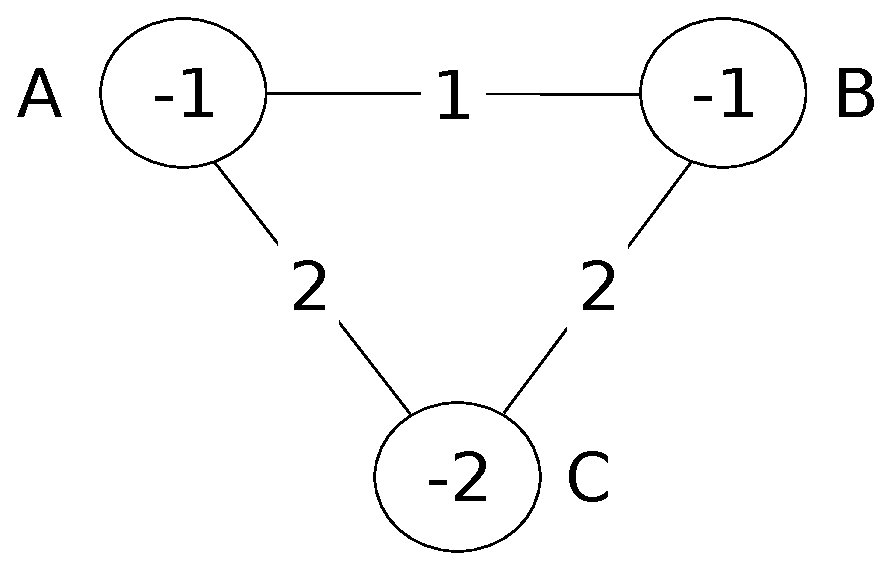
\includegraphics{img/nand.eps}
	}
\end{center}
	\caption[\texttt{NAND} Graph]{Graphical representation of the Hamiltonian implementing the logic of a \texttt{NAND} gate.  Each of the vertices is a spin and the number inside is the field value on that spin; each edge is the coupling value between the respective vertices.  The top two spins are the input spins, while the bottom is the output.  Each ground state of this Hamiltonian enforces the logic $C = \neg(A \wedge B)$.}
	\label{fig:nand_graph}
\end{figure}

Simply evaluating the Hamiltonian depicted in Figure \ref{fig:nand_graph} will reproduce the entire truth table of the \texttt{NAND} gate.  Usually computing the entire truth table of our circuit is not what we want; we want to specify some input and get only the corresponding output.  This is done by a process called \emph{clamping}.  

Clamping manipulates a Hamiltonian to mimic the effect of fixing certain spins to specified values.  This is done in several steps.  First, we select a value $C$ for the spin $s$ to be clamped to.  $s$ is then removed from the Hamiltonian; each coupling between $s$ and a different spin $d$ is removed, and the value $Cs$ is added to the field on spin $d$.  This changes the energy spectrum associated with spin $d$ to match what it would be were $s$ still in the Hamiltonian with the value $C$.

For example, in the \texttt{NAND} Hamiltonian from Figure \ref{fig:nand_graph}, clamping the spin $C$ to $+1$ or $true$  would result in the field terms on $A$ and $B$ becoming $-1 + 1\times2 = 1$.  The final Hamiltonian would then be fields of $+1$ on spins $A$ and $B$ and a coupling between them also with strength $+1$, while $C$ would be gone.  The ground state energy of this Hamiltonian is $-1$, with three ground states corresponding to either spin $A$ or $B$ up with the other down, or both spins down.  The only state of the two spins not in the ground state degeneracy is the state $A = B = \uparrow$; this is the only input to a \texttt{NAND} gate that does not result in a \texttt{true} output, and we restricted this Hamiltonian to values of $A$ and $B$ for which $C$ is \texttt{true}.

The notable feature of this example is that we clamped what is normally an \emph{output} spin.  Because quantum mechanics is reversible, all of our computations must be as well; this means AQC Hamiltonians are symmetric between input and output.  We take advantage of this when designing our circuits: any circuit that computes a function $f$ also computes its inverse $f^{-1}$.  Thus a circuit that computes multiplication is also a circuit that computes integer factorization, depending on whether the spins corresponding to the factors or the multiplicand are clamped.  Since we can construct a classical multiplication circuit out of a polynomial number of \texttt{NAND} gates, we can also construct an AQC integer factorization circuit out of a polynomial number of quantum \texttt{NAND} gates.

\section{Adiabatic Evolution}
Once we have a Hamiltonian whose ground state encodes the problem we would like to solve, we need to set up the evolution.  The Adiabatic Theorem lets us transition from the ground state of one Hamiltonian to another, so we need an initial Hamiltonian.  In general almost any Hamiltonian of which we know the ground state will work.  For simplicity we use the following initial Hamiltonian:
\begin{equation}
	\ham_i = \sum_i^N B \sigma_i^x
\end{equation}
where $B$ is some large constant.  This Hamiltonian has as it's ground state all the spins pointed along the (negative) x-axis (or equivalently, an equal superposition of $\ket{\pm z}$).  This is easy to prepare by applying a large magnetic field along the negative x direction.
Once we've assembled both our initial and final Hamiltonians, we can conduct the evolution.  We call the total Hamiltonian $H_{tot}$, and it is simply the sum of the initial and final Hamiltonian:

\begin{equation}
	\ham_{tot} = A(t)\ham_i + B(t)\ham_f
\end{equation}

where $A(t)$ and $B(t)$ are dimensionless functions of time such that $A(0) = B(T) = 1$ and $A(T) = B(0) = 0$ where $T$ is the final annealing time; this ensures that at $t = 0$ the Hamiltonian is equal to $H_i$ and at $t = T$ the Hamiltonian is equal to $H_f$.  Then the functions $A$ and $B$ describe the \emph{evolution path}.  Combining the evolution path with the speed at which the Hamiltonian is changing (or just the speed), that is $\frac{\partial A}{\partial t}$ and $\frac{\partial B}{\partial t}$, gives us the evolution trajectory.  

Given a ground state of $\ham_{tot}$, $\ket{\psi_{gs}}$, the \emph{fidelity} is the probability of measuring $\psi_{gs}$, or $|\braket{\psi(T)|\psi_{gs}}|^2$.  If there are $N$ correct answer to our computation, and thus $\ket{\psi_N}$ degenerate ground states, the fidelity is defined as

\begin{equation}
	F = \sum_{i=0}^N \braket{\psi(T)|\psi_i}
\end{equation}

For a perfectly annealed system, the fidelity should go to one as the annealing time increases.  Since any real annealing will not be in the infinite anneal time limit, in practice our fidelity values are restricted to be $\leq 1$.  The closer the fidelity is to 1, the more likely our computation is to succeed.  We will use the fidelity later in the experimental results section to evaluate how close we get to ideal AQC.

For a purely quantum mechanical system described by the Hamiltonian $\ham_{tot}$, the evolution trajectory completely determines the fidelity.
The simplest and most obvious trajectory is $A(t) = 1 - t/T$ and $B(t) = t/T$ at a constant speed, or a straight line path through Hamiltonian space.
There is no particular reason that a straight line from $(A=1,B=0)$ to $(A=0,B=1)$ should maximize the fidelity; indeed, because moving away from the origin in Hamiltonian space scales the Hamiltonian and its derived quantities up (including the energy gap), and the adiabatic condition is stated in terms of the energy gap, we expect that some more complicated curve through Hamiltonian space, potentially including changing the evolution speed, will give the best results.

However, in this work we restrict ourselves to evaluating straight line paths through Hamiltonian space due to the adiabatic quantum computer we eventually run jobs on being limited in this manner (see Chapter \ref{chap:machine}).

\section{Simulating AQC}
For small Hamiltonian we can simulate directly the process of quantum annealing by integrating the Schr\"odinger equation. For time dependent Hamiltonians such as ours, the general form of the Schr\"odinger equation is 

\begin{equation}
	i\hbar\frac{\partial}{\partial t} \Psi = \ham\Psi
\end{equation}

this is a linear partial differential equation which can be easily solved by numerical methods.  Using a fourth order Runge-Kutta method\cite{comp_book} we can find the overlap between the ground state $\ket{\psi_f}$ and the current state $\ket{\psi(t)}$ and plot this as a function of the annealing parameter.  Figure \ref{fig:simulate} shows the results of one such simulation.  This shows an eight spin Hamiltonian annealed with linear control parameters $A(t) = 1-t/T$ and $B(t) = t/T$.  The features correspond to what we expect from the adiabatic theorem: the fidelity starts low and climbs as the system evolves.  It does not reach one as we are not in the adiabatic limit because we are annealing for only a finite time.  We expect to see similar results to the one shown here from experimental data; deviations will show us how far our experiments depart from the assumptions of AQC.
\begin{figure}
	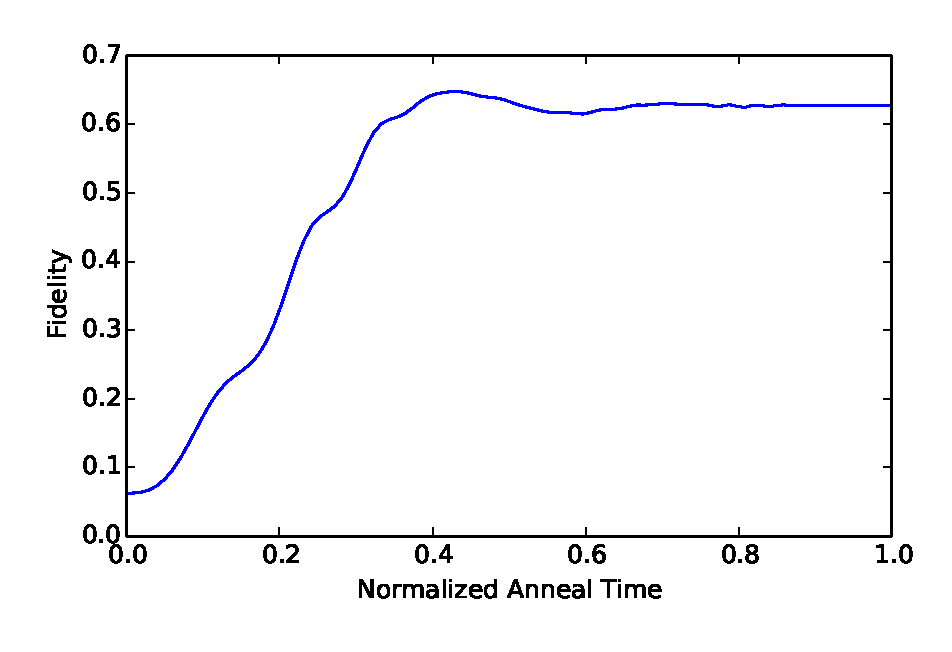
\includegraphics{img/simulate.eps}
	\caption[Simulated AQC]{Numerical simulation of adiabatic evolution by integrating the Schr\"odinger equation.}
	\label{fig:simulate}
\end{figure}
